\documentclass[14pt,letterpaper]{article}
\usepackage[margin=2cm,includefoot]{geometry}
\usepackage[spanish]{babel}

\usepackage[%  
    colorlinks=true,
    pdfborder={0 0 0},
    linkcolor=blue
]{hyperref}

\usepackage{xcolor}
\usepackage{amsmath}
\usepackage{multicol}
\usepackage{graphicx}
\usepackage{qtree}
\usepackage{tikz}

\usepackage{imakeidx}
\makeindex[columns=3, title=Alphabetical Index, intoc]

\graphicspath{ {./img/} }

\title{Programa 02 \\ Approx Subset-Sum}
\author{Diego Méndez Medina}
\date{}


\begin{document}

\ttfamily
\maketitle
\rmfamily

\tableofcontents
\printindex
\clearpage

\section{{\sc Introducción}}
Resolvi approx subsetsum según lo descrito en el libro {\it Introduction to
  Algorithms}.

En la carpeta {\it src} se encuentra el archivo {\it Readme.org} donde hay
instrucciones para compilar y ejecutar el programa.

\section {\sc Sample1}

  Es el ejemplo enunciado en el libro.
  \begin{figure}[h]
    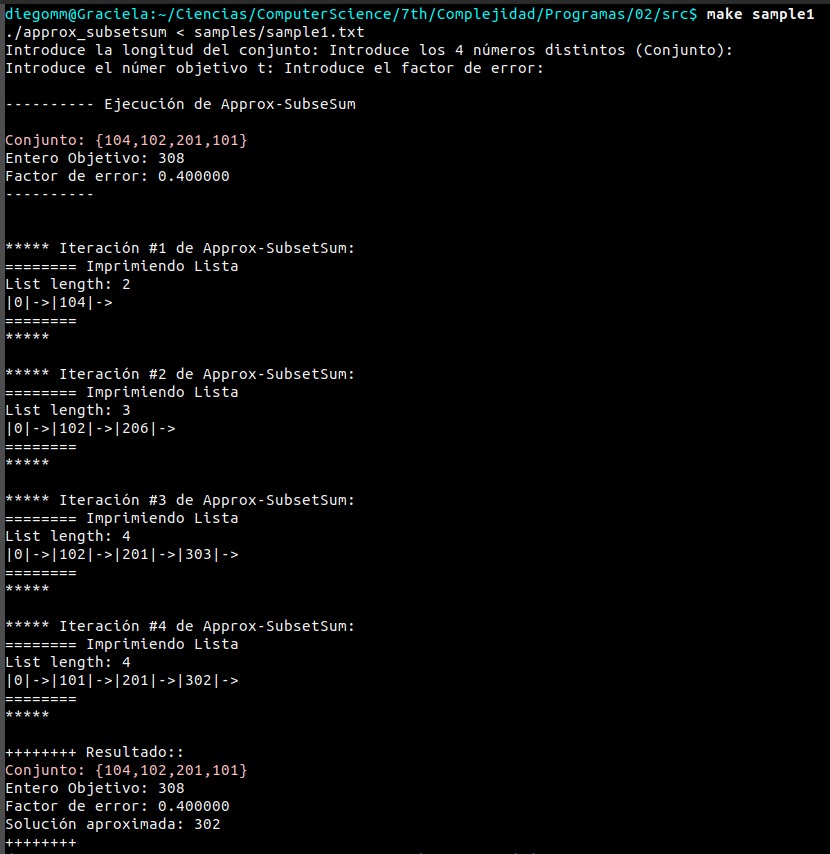
\includegraphics[width=15cm]{sample1.png}
    \centering
  \end{figure} 

  \clearpage
\section {\sc Sample2}

Primera (1 de 2) captura de la ejecución.

  \begin{figure}[h]
    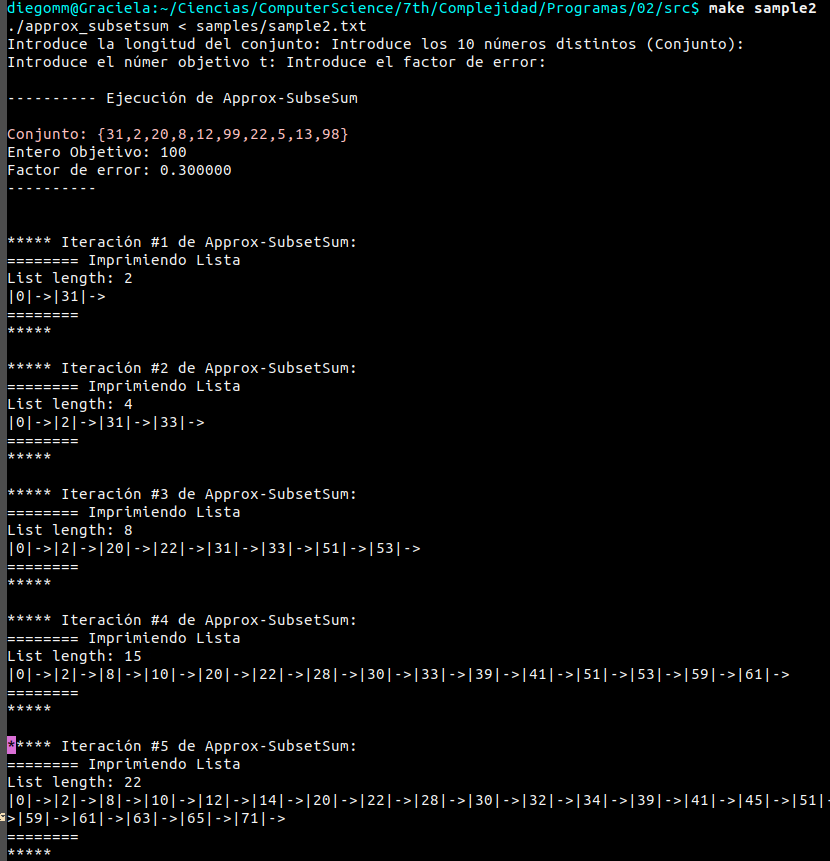
\includegraphics[width=15cm]{sample2_1.png}
    \centering
  \end{figure}

  \clearpage
  Última (2 de 2) captura de la ejecución.
  \begin{figure}[h]
    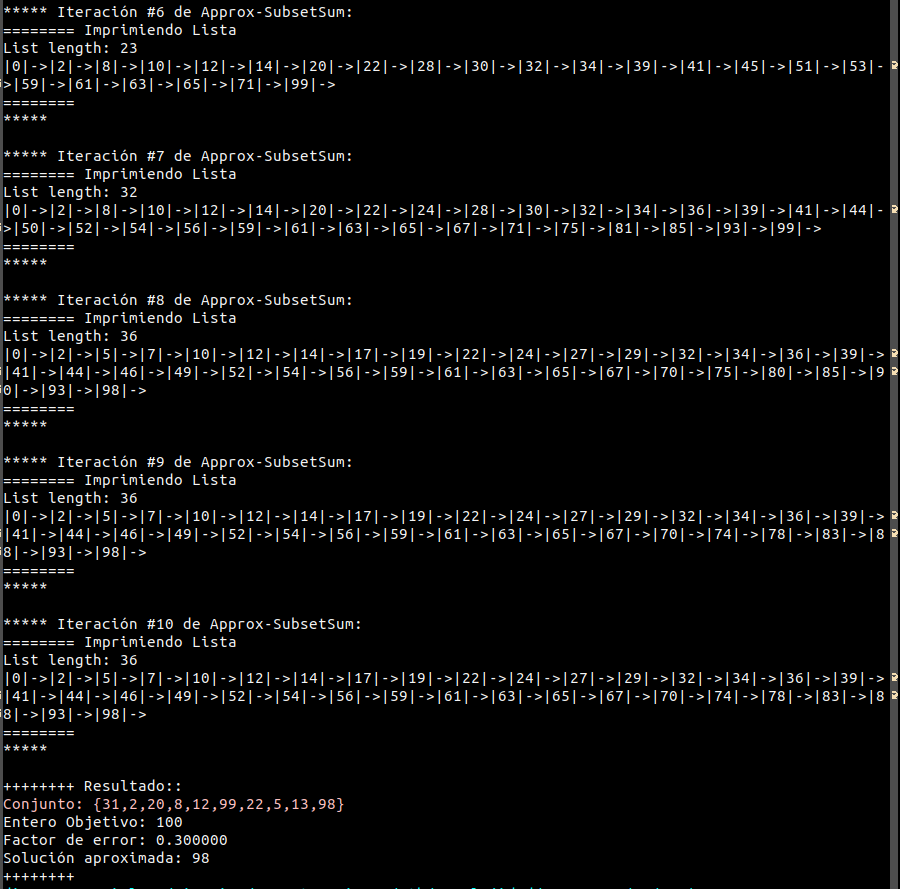
\includegraphics[width=15cm]{sample2_2.png}
    \centering
  \end{figure}
  \clearpage
  \section{\sc Sample3}
  
  \begin{figure}[h]
    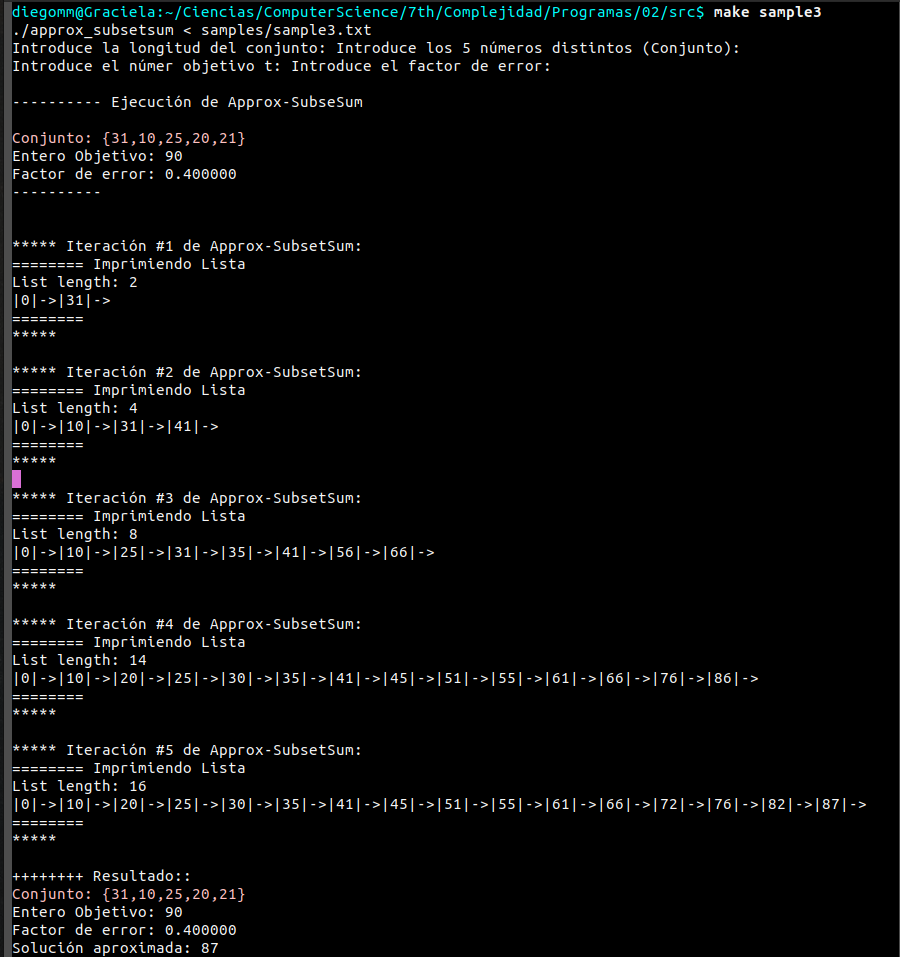
\includegraphics[width=15cm]{sample3.png}
    \centering
  \end{figure}
  \clearpage
  \section {\sc Sample4}
    Primer (1 de 4) captura de la ejecución.
  \begin{figure}[h]
    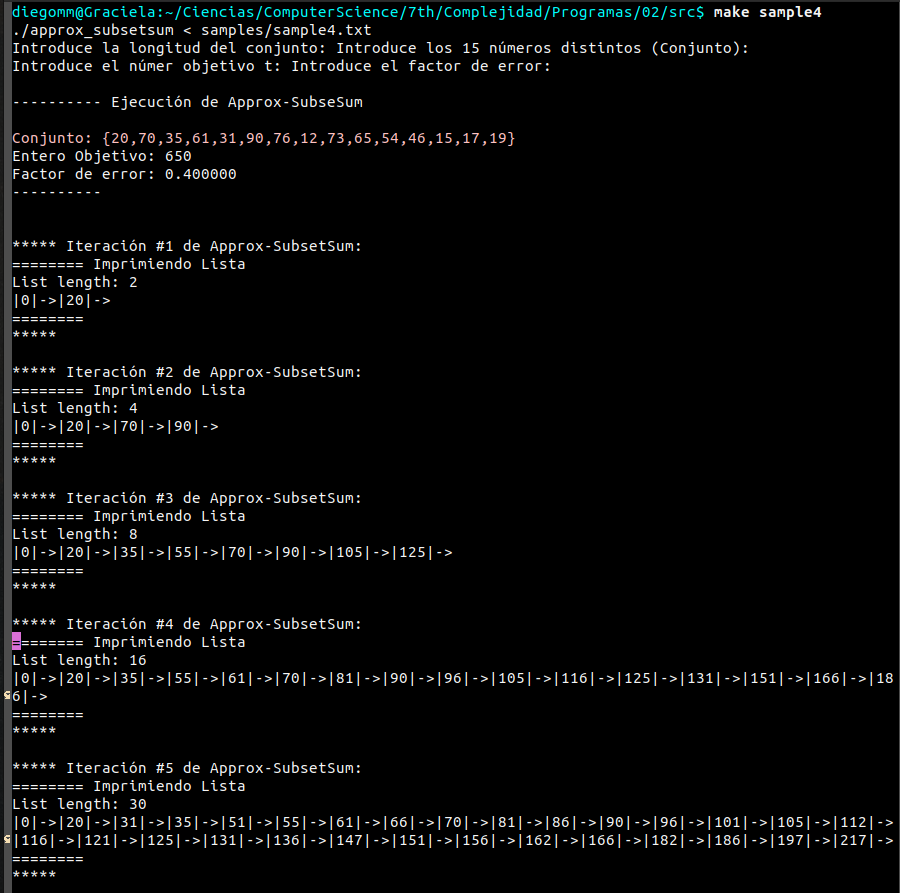
\includegraphics[width=15cm]{sample4_1.png}
    \centering
  \end{figure}
  \clearpage
  Segunda (2 de 4) captura de la ejecución.
  \begin{figure}[h]
    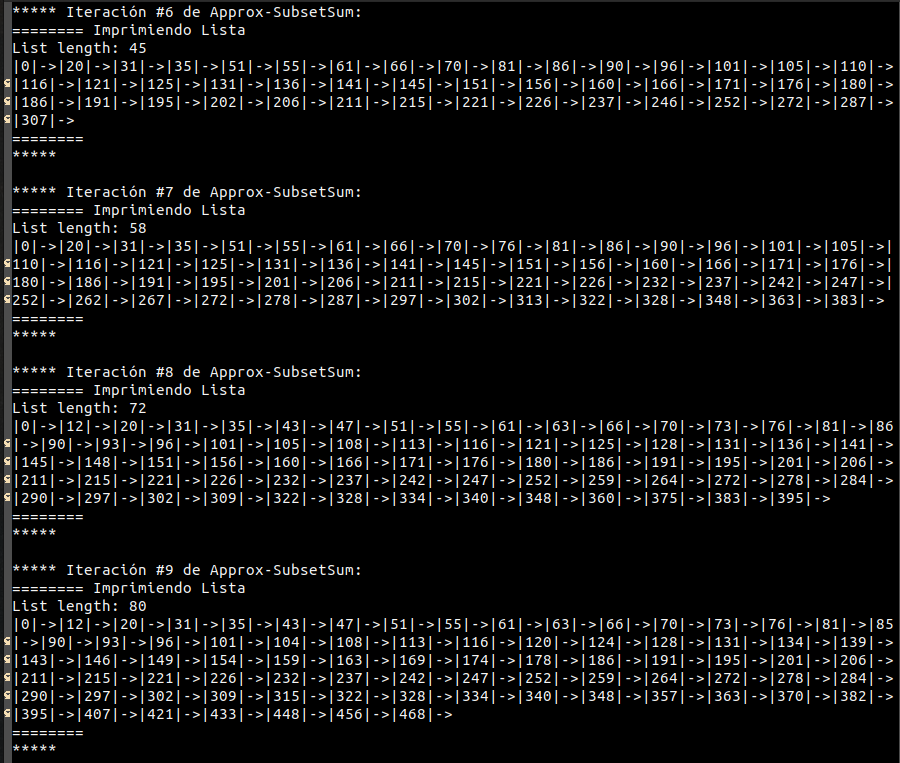
\includegraphics[width=15cm]{sample4_2.png}
    \centering
  \end{figure}
  \clearpage
  Tercer (3 de 4) captura de la ejecución.
  \begin{figure}[h]
    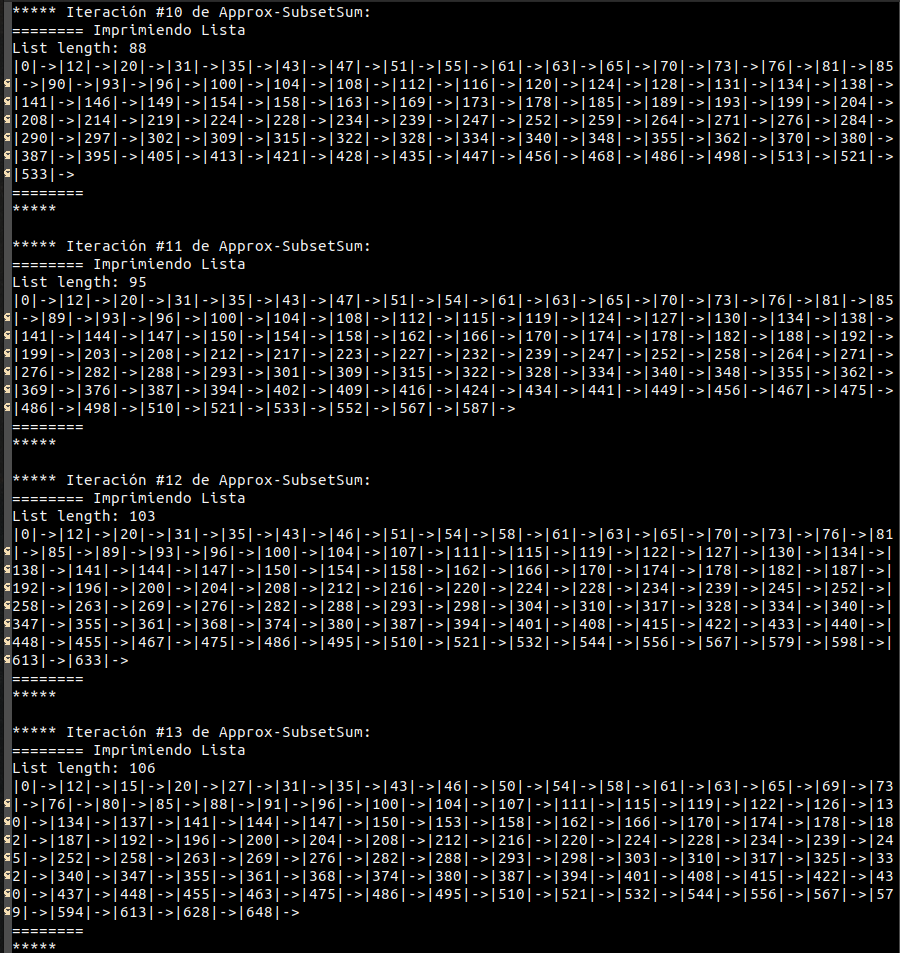
\includegraphics[width=15cm]{sample4_3.png}
    \centering
  \end{figure}
  \clearpage
  Última (4 de 4) captura de la ejecución.
  \begin{figure}[h]
    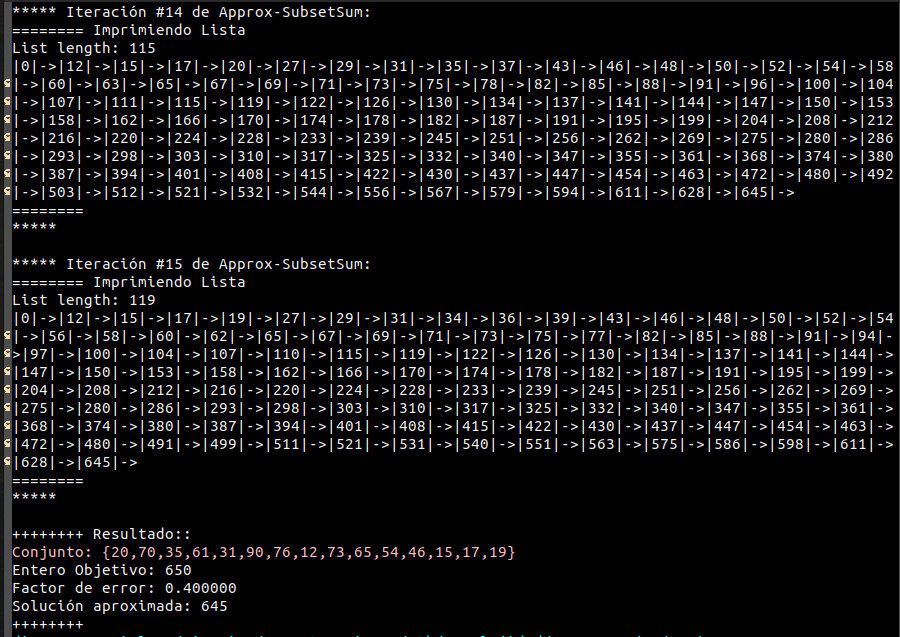
\includegraphics[width=15cm]{sample4_4.png}
    \centering
  \end{figure}
  \clearpage
\section {\sc Sample5}  
  Primer (1 de 2) captura de la ejecución.
  \begin{figure}[h]
    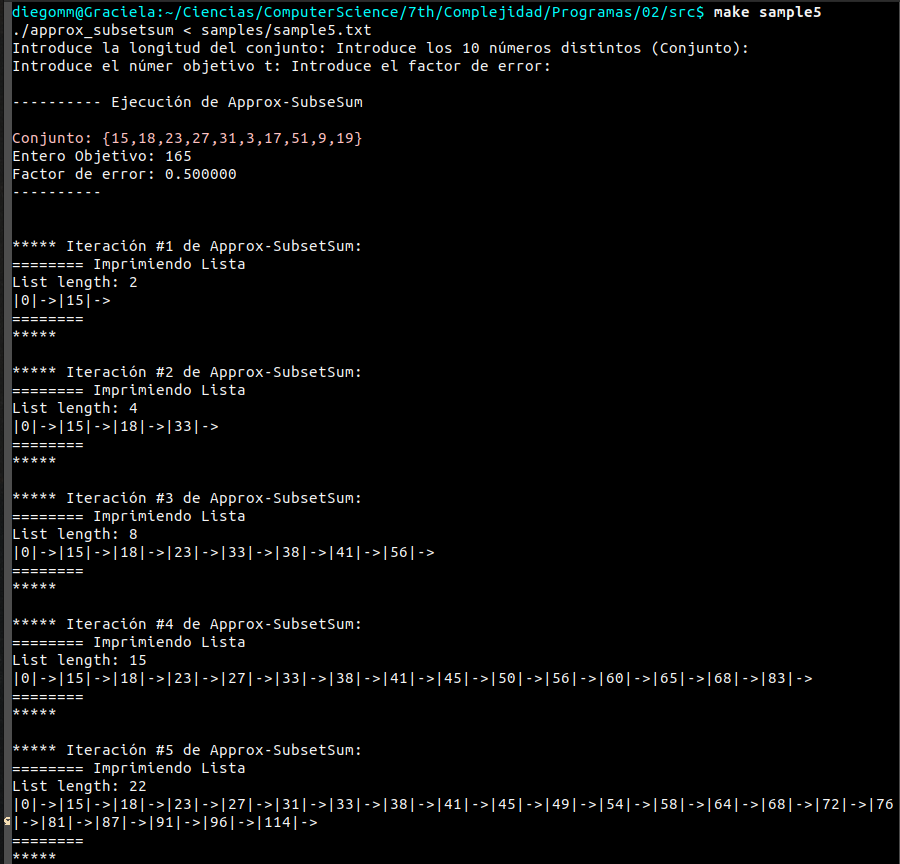
\includegraphics[width=15cm]{sample5_1.png}
    \centering
  \end{figure}
  \clearpage
  Última (2 de 2) captura de la ejecución.
  \begin{figure}[h]
    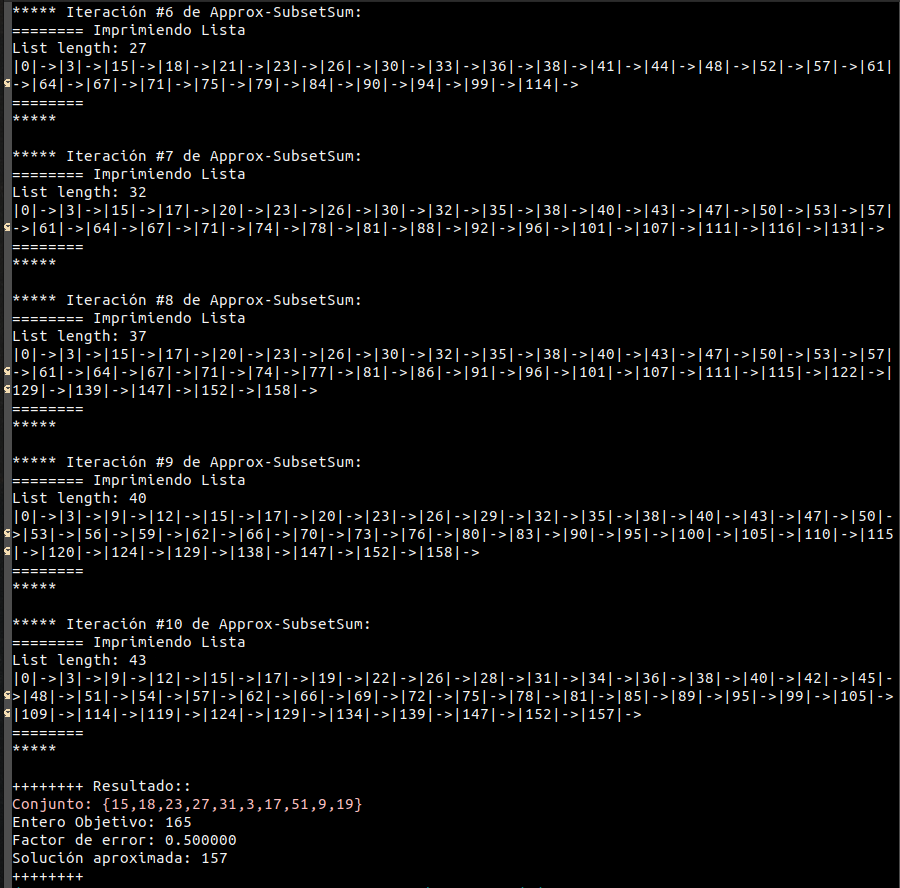
\includegraphics[width=15cm]{sample5_2.png}
    \centering
  \end{figure}
  \clearpage
\end{document}



